\chapter{Conclusion and Discussion}
\label{conclusion}

This thesis presents evidence for electroweak single top quark production at the Tevatron. An analysis of nearly $1$~fb$^{-1}$ of Run~II data using the matrix element method to select single top quark-like events measures the combined $s+t$-channel production cross section to be
$$
\sigma\left({\ppbar}{\rargap}tb+tqb+X\right)
= 4.6 ^{+1.8}_{-1.5}~{\rm pb},
$$

\noindent where the probability of a background fluctuation is $0.21\%$, which corresponds to a Gaussian equivalent signal significance of $2.9\sigma$. This analysis is one of three single top searches performed by the $\dzero$~collaboration. The first analysis using boosted decision trees measures a combined $s+t$ cross section of $4.9\pm1.4$~pb with a signal significance of 3.4$\sigma$, while the second analysis uses Bayesian neural networks and measures a cross section of $5.0\pm1.9$~pb at 2.4$\sigma$ signal significance. The results of these three analyses were recently accepted for publication by Physical Review Letters~\cite{Abazov:2006gd}. More recently the three results were combined using the BLUE (Best Linear Unbiased Estimator)~\cite{1988NIMPA.270..110L} method; this resulted in a measured cross section of $4.8\pm1.3$~pb with $3.5\sigma$ signal significance~\cite{comb}. The cross sections from the three analyses as well as the combination are shown in Fig.~\ref{singletopanalysis}, where they are also compared with two next-to-leading order single top cross section calculations.

\begin{figure}[!h!tbp]
\begin{center}
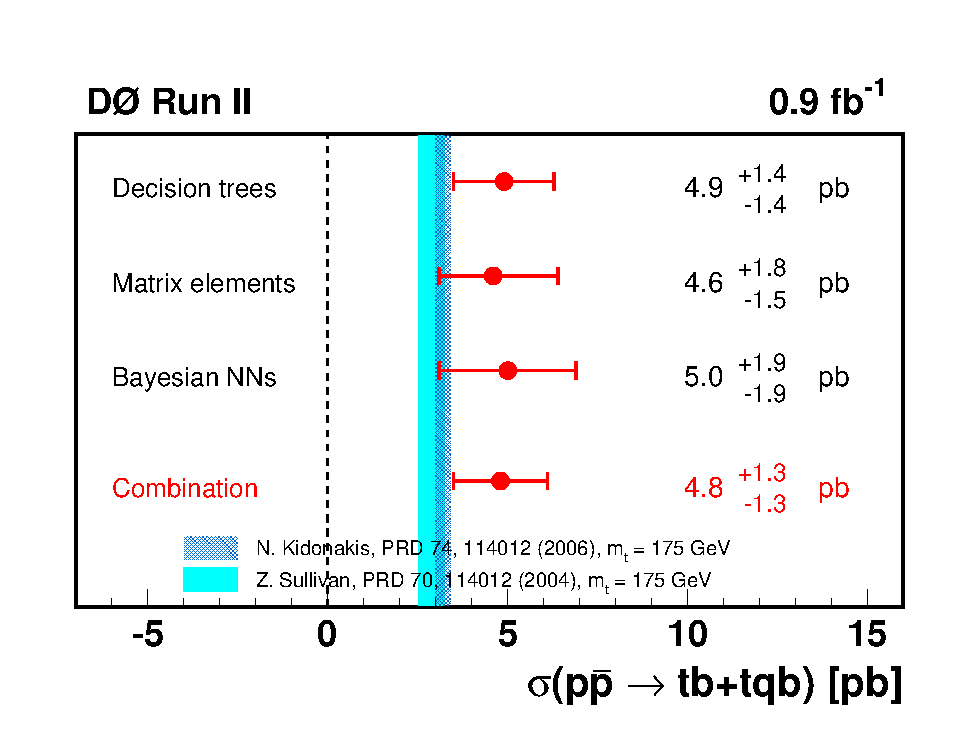
\includegraphics[width=0.75\textwidth]{eps/Conclusion/ResultsComb.eps}
\end{center}
\vspace{-0.1in}
\caption{Results from the three single top quark analyses and the combined analysis compared with two NLO cross section calculations~\cite{comb}.}
\label{singletopanalysis}
\end{figure}

Several improvements to the matrix element analysis presented in this thesis are currently underway. First is the addition of a $\ttbar$~matrix element in the discriminant definition. This should dramatically enhance the signal significance in events with three jets where the $\ttbar$~background contribution is substantial. The second improvement is the use of the muon charge from a semi-leptonic $B$ decay to weight the jet-parton assignment of jets to $b$ and $\bar{b}$ quarks, while the third is the addition of the neural network $B$-tagging algorithm in the discriminant definition. Events with jets that are very $B$-jet like will receive a higher weight from background processes involving $b$~quarks \mbox{(e.g. $Wb\bar{b}$)} while the remaining events will receive a higher weight from processes involving light quarks \mbox{(e.g. $Wgg$ and $Wcg$)}.

$\dzero$ has already recorded more than $2$~fb$^{-1}$ of Run~II data. With this increased dataset several important measurements are possible. The first is an individual measurement of the $s$-channel and $t$-channel cross sections. Each production process is sensitive to different new physics models making a determination of the cross section for each channel an important test for physics beyond the Standard Model. Another important measurement using this dataset is a precise determination of $|V_{tb}|$. The current uncertainty on the combined single top cross section is $\sim30\%$, which leads to an uncertainty on $|V_{tb}|$ of $\sim20\%$. With this increased dataset the expected error on $|V_{tb}|$ will decrease to $15\%$. 

A precise measurement of the single top quark production cross section is also important because single top events are one of the largest backgrounds for Higgs production. At the Tevatron one of the most sensitive channels for a low mass Higgs is $W$-associated Higgs production ($WH$). The $WH$ production cross section for $m_{H}=115$~GeV is nearly one-tenth of the single top cross section. Using the full Run~II dataset and employing advanced multivariate analysis techniques such as the method described in this thesis, $\dzero$ hopes to find evidence for the Higgs boson before the start of the Large Hadron Collider era.

The analysis presented in this thesis has shown that with a detailed understanding of the detector apparatus, an advanced multivariate technique to reduce backgrounds, and a sophisticated statistical analysis of the dataset, the measurement of a process which occurs in 1 out of every 10 billion collisions at the Tevatron is possible. With an increased dataset of $3-4$~fb$^{-1}$ a $5\sigma$ observation of single top production will be possible, thereby providing a stringent test of the Standard Model and possibly establishing the presence of new physics.